\documentclass[10pt]{article}
\usepackage[letterpaper,margin=0.725in]{geometry}

\usepackage{fancyhdr}
\usepackage{amsmath}
\usepackage{mathtools}
\usepackage{hyperref}
\usepackage[english]{babel}
\usepackage{graphicx}
\usepackage{float}
\usepackage{caption}
\usepackage{amssymb}
\usepackage{caption}
\usepackage{amstext} % for \text macro
\usepackage{array}   % for \newcolumntype macro
\allowdisplaybreaks

\usepackage[T1]{fontenc}
\usepackage[numbered,framed]{matlab-prettifier}

\hypersetup{ colorlinks=true, linkcolor=blue}

\DeclareMathOperator{\atantwo}{atan2}
\newcolumntype{C}{>{$}c<{$}} % math-mode version of "l" column type

\pagestyle{fancy}
\lhead{RBE 500 - PA \#3 \newline Team 2: Peter Campellone, Aislin Hanscom, Christopher Poole}
\rhead{Due: 7/27/2021}

\begin{document}

\setlength{\abovedisplayskip}{6pt}
\setlength{\belowdisplayskip}{3pt}
\setlength{\abovedisplayshortskip}{4pt}
\setlength{\belowdisplayshortskip}{4pt}

\textbf{Package overview:}
\begin{itemize}
	\item Inside \texttt{catkin\_ws/src}, the main package is \texttt{scara\_robot}. It does not directly contain any nodes or launch files, but is a way to organize all of the other nodes.
	\begin{itemize}
		\item New packages:
		\begin{itemize}
			\item The \texttt{scara\_pd\_controller} package implements a proportional and derivative controller for the three controllable joints: joint 1 (revolute), 2 (revolute), and 5 (prismatic joint). The controller functions by reading the current joint position using the \\ \texttt{gazebo/get\_joint\_properties} service, calculating the necessary input into the joint, and applying the input force using the \texttt{gazebo/apply\_joint\_effort} service. The controller receives the desired reference position using a custom service message under \texttt{scara/JointControlReference}.
			\item The \texttt{scara\_velocity\_controller} package aims to control the end effector velocity given a global reference. It calculates the necessary joint rates using the \texttt{scara\_velocity\_kinematics} package and controls them individually using a set of PD controllers.
			\item The \texttt{scara\_velocity\_kinematics} package contains two services that calculate the forward and inverse Jacobian for the manipulator. It also calculates the necessary joint rates given a current position and desired end effector velocity or the end effector velocity given the current position and current joint rates.
		\end{itemize}
		
		\item Old packages used (from PA \#1):
		\begin{itemize}
			\item The \texttt{scara\_gazebo} package includes the launch files for the gazebo world.
			\item The \texttt{scara\_description} package includes the URDF files for the robot as well as the rviz launch files.
		\end{itemize}
	\end{itemize}
\end{itemize}
\vspace{0.5cm}

\textbf{Problems:}

The following coordinate frame definitions will be used for all parts:

\begin{figure}[H]
	\centering
	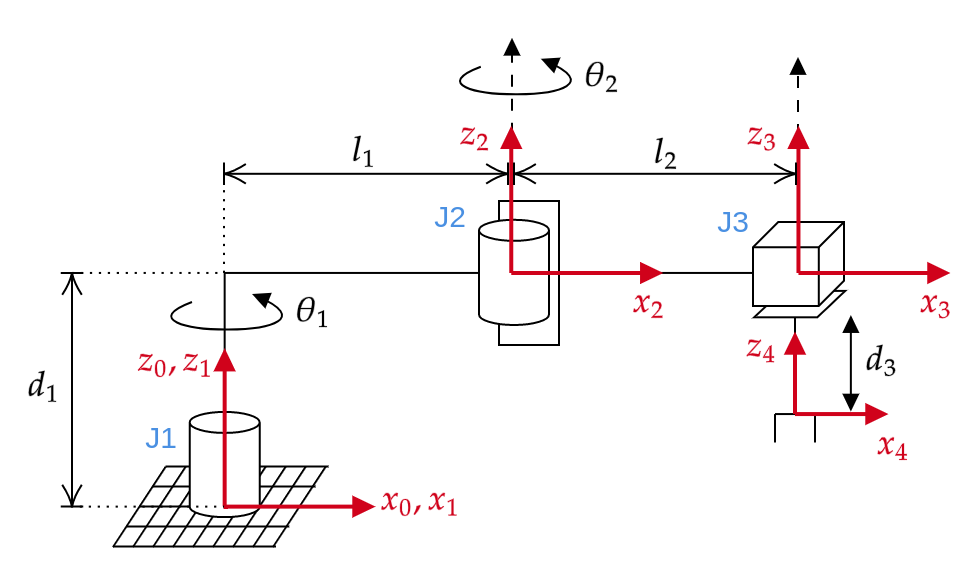
\includegraphics[width=0.6\textwidth]{figures/rrp_manipulator_reference_frames.png}
\end{figure}

\begin{enumerate}
	\item Velocity Level Kinematics: Implement a node with two services. One takes joint velocities and converts them to end effector velocities, and the second one takes end effector velocities and converts them to joint velocities.
	\\
	
	The work to derive the equations is attached in the submission.
	\\
	
	To run the node:
	
	\begin{enumerate}
		\item \texttt{catkin\_make}
		\item \texttt{source devel/setup.bash}
		\item \texttt{rosrun scara\_velocity\_kinematics velocity\_kinematics.py}
		\item In a new window, \texttt{rosservice call /scara/ForwardJacobianCalculation} and double tab complete
		\item In a new window, \texttt{rosservice call /scara/InverseJacobianCalculation} and double tab complete
	\end{enumerate}
	
	\item Extend the position controller in Part 2 to all the joints. (don't forget to revert the joint types.) Move the robot to a position that is significantly away from singular configurations using you position controllers
	\\
	
	First the revolute joints were reverted back to non-fixed joints in the gazebo XACRO file:
	
\begin{lstlisting}[style=Matlab-editor,basicstyle=\mlttfamily,escapechar=`]
<joint name="joint1" type="revolute">
	<parent link="link1"/>
	<child link="link2"/>
	<origin xyz="0 0 ${height1 - axel_offset}" rpy="0 0 1.570796"/>
	<axis xyz="0 0 -1"/>
	<limit effort="100" lower="-3.14" upper="3.14" velocity="1"/>
	<dynamics damping="0.7"/>
</joint>
...
<joint name="joint3" type="revolute">
	<parent link="link3"/>
	<child link="link4"/>
	<origin xyz="0 1.5 2.5" rpy="1.57 0 0"/>
	<axis xyz="0 0 1"/>
	<limit effort="100" lower="-3" upper="3" velocity="1"/>
	<dynamics damping="0.7"/>
</joint>
\end{lstlisting} 
	
	The PD position controller from PA2 was expanded to control the revolute joints (referred to as joints 1 and 3 in gazebo because of the fixed joints). The following equation was used:
	
	\begin{align*}
		C(s) = k_p + k_d s \Rightarrow c(t) = k_p E + k_d \frac{dE}{dt}
	\end{align*}
	
	The controller function from PA2 was already made to take in arbitrary current positions, desired positions, gains, and the joint name, but minor changes were made to the way the error is passed into the function:
		
\begin{lstlisting}[style=Matlab-editor,basicstyle=\mlttfamily,escapechar=`]
def pd_control(joint, pos_cur, pos_des, kp, kd, err_old):
	err = pos_des - pos_cur
	d_err = (err - err_old)/(1/rate)
	f = -(kp*err + kd*d_err)
	
	if debug == True:
		print("err = %f,  d_err = %f" % (err, d_err))
		print("pos_des = %f, pos_cur = %f" % (pos_des, pos_cur))
		print("Sending joint force f = [%f]" % (f)) # printing calculated values to terminal
	
	je_service = rospy.ServiceProxy('/gazebo/apply_joint_effort', ApplyJointEffort)
	zero_time = rospy.Time()
	tick = rospy.Duration(0, int((1/rate)*10**9))
	je_service(joint, f, zero_time, tick)
	
	if print_to_file == True:
		file1.write("%s,%f,%f,%f,%f\n" % (joint,pos_cur, pos_des,f,1/rate)) 
	
	return err
\end{lstlisting} 

	The function created to request the joint position was also expanded to work for all three joints. This also calls the PD controller function using the current joint position, desired joint position, gains, and previous loop error (for the derivative calculation):
		
\begin{lstlisting}[style=Matlab-editor,basicstyle=\mlttfamily,escapechar=`]
def request_joint_status(joint):

	joint_stauts = rospy.ServiceProxy('/gazebo/get_joint_properties', GetJointProperties)
	resp = joint_stauts(joint)
	
	joint_pos = resp.position[0]
	
	if debug == True:
		print("\n\nReceived %s position: [%f] (meters)" % (joint,joint_pos)) # printing received data to terminal
	
	if joint == 'joint1':
		E_old[0] = pd_control('joint1', -joint_pos, -th1_des, kp[0], kd[0], E_old[0])
	
	if joint == 'joint3':
		E_old[1] = pd_control('joint3', -joint_pos, th2_des, kp[1], kd[1], E_old[1])
	
	if joint == 'joint5':
		E_old[2] = pd_control('joint5', -joint_pos, d3_des, kp[2], kd[2], E_old[2])
	
	return resp
\end{lstlisting} 

	The reference position service message file was updated to include the positions of the revolute joints:
	
\begin{lstlisting}[style=Matlab-editor,basicstyle=\mlttfamily,escapechar=`]
float64 th1_des
float64 th2_des
float64 d3_des
---
float64 success
\end{lstlisting}

	The service handler function was also updated to store the desired positions for the revolute joints:
	
\begin{lstlisting}[style=Matlab-editor,basicstyle=\mlttfamily,escapechar=`]
def service_handle(data):
	global th1_des
	global th2_des
	global d3_des
	
	th1_des = data.th1_des
	th2_des = data.th2_des
	d3_des = data.d3_des
	
	if debug == True:
		print("\nReceived reference positions [th1,th2,d3] = [%f,%f,%f]" % (th1_des,th2_des,d3_des)) # printing converted values to terminal
	
	if d3_des >= 0 or d3_des <=1:
		success = True
	else:
		success = False
	
	return success
\end{lstlisting}	

	Lastly, the server loop was updated to poll the positions of the revolute joints (which in turns calls the controller of each joint each cycle):
	
\begin{lstlisting}[style=Matlab-editor,basicstyle=\mlttfamily,escapechar=`]
while not rospy.is_shutdown():
	request_joint_status('joint1')
	request_joint_status('joint3')
	request_joint_status('joint5')
	r.sleep()
\end{lstlisting}	


	When the controller begins, it commands the joints to the home position. The reference position was then set to a two different non-zero positions to show the controller functioning:
	
	\begin{minipage}[H]{0.45\textwidth}
		\centering
		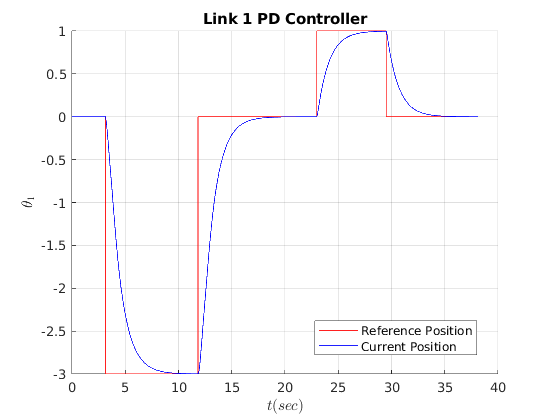
\includegraphics[width=0.95\textwidth]{figures/link1-pd-plot1.png}
	\end{minipage}
	\begin{minipage}[H]{0.45\textwidth}
		\centering
		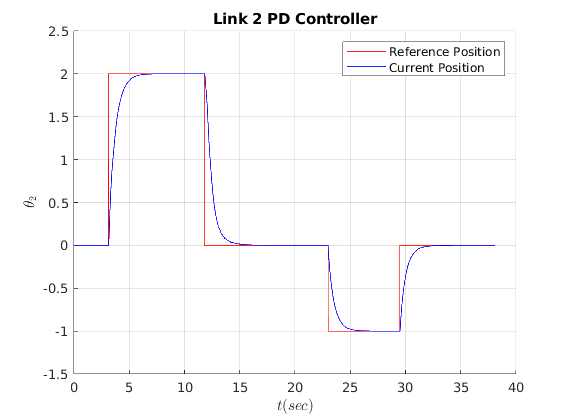
\includegraphics[width=0.95\textwidth]{figures/link2-pd-plot1.png}
	\end{minipage}

	\begin{figure}[H]
		\centering
		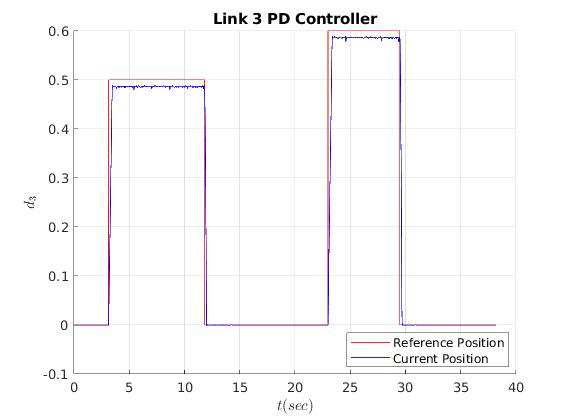
\includegraphics[width=0.45\textwidth]{figures/link3-pd-plot1.png}
	\end{figure}
	
	We can see that the controllers are functioning for all three joints. Links 1 and 2 have a slower response than Link 3 because of lower gains. Link 3 required higher gains to overcome the constant gravity force. If the proportional gain for link 1 and 2 was increased too much more, it would also increase the overshoot. The derivative gain could then be increased as well to combat this, but it could lead to system instability.
	\\

	To run the controller:
	
	\begin{enumerate}
		\item \texttt{catkin\_make}
		\item \texttt{source devel/setup.bash}
		\item \texttt{roslaunch scara\_gazebo scara\_world.launch}
		\item In a new window, \texttt{rosrun scara\_pd\_controller pd\_control.py}. The controller will begin controlling all joints to their home position ($\theta_1 = \theta_2 = d_3 = 0$).
		\item In a new window, \texttt{rosservice call /scara/JointControlReference "th1\_des: X.XX th2\_des: X.XX d3\_des: X.XX"} where \texttt{X.XX} is any number between $-\pi$ and $\pi$ for the revolute joints and 0 and 1 for the prismatic joint.
	\end{enumerate}
	
	\item Write velocity controllers for all the joints. For tuning the controller gains, you might need to fix the joints rather than the joint of consideration. Don't forget to revert the joint type to movable ones once you are done.
	\\
	
	The velocity controllers are written in the \texttt{velocity\_control} function within the velocity controller node:

\begin{lstlisting}[style=Matlab-editor,basicstyle=\mlttfamily,escapechar=`]
def velocity_control(joint, vel_cur, vel_des, kp, kd, err_old):
	
	err = vel_des - vel_cur
	d_err = (err - err_old)/(1/rate)
	
	f = -(kp*err + kd*d_err)
	
	if debug == True:
		print("\nerr = %f,  d_err = %f" % (err, d_err))
		print("vel_des = %f, vel_cur = %f" % (vel_des, vel_cur))
		print("Sending joint force f = [%f]" % (f)) # printing calculated values to terminal
	
	je_service = rospy.ServiceProxy('/gazebo/apply_joint_effort', ApplyJointEffort)
	zero_time = rospy.Time()
	tick = rospy.Duration(0, int((1/rate)*10**9))
	je_service(joint, f, zero_time, tick)
	
	if print_to_file == True:
		file1.write("%s,%f,%f,%f,%f\n" % (joint,vel_cur, vel_des,f,1/rate)) 
	
	return err
\end{lstlisting}	

	The main server loop is as such:
	
\begin{lstlisting}[style=Matlab-editor,basicstyle=\mlttfamily,escapechar=`]
while not rospy.is_shutdown():

	request_joint_status('joint1')
	request_joint_status('joint3')
	request_joint_status('joint5')
	
	# calculate current q_dot
	q_dot_cur = (joint_pos_cur - joint_pos_old)/(1.0/rate)
	
	th1 = joint_pos_cur[0]
	th2 = joint_pos_cur[1]
	d3 = joint_pos_cur[2]
	
	jac_service = rospy.ServiceProxy('scara/InverseJacobianCalculation', ee_to_joint_velocity)
	jac_resp = jac_service(th1,th2,d3,x_dot_des,y_dot_des,z_dot_des)
	
	q_dot_des[0] = jac_resp.th1_dot
	q_dot_des[1] = jac_resp.th2_dot
	q_dot_des[2] = jac_resp.d3_dot
	
	# invoke controller and set return = q_dot_err for next control loop
	q_dot_err[0] = velocity_control('joint1', q_dot_cur[0], q_dot_des[0], kp[0], kd[0], q_dot_err[0])
	q_dot_err[1] = velocity_control('joint3', q_dot_cur[1], q_dot_des[1], kp[1], kd[1], q_dot_err[1])
	q_dot_err[2] = velocity_control('joint5', q_dot_cur[2], q_dot_des[2], kp[2], kd[2], q_dot_err[2])
	
	joint_pos_old[0] = joint_pos_cur[0]
	joint_pos_old[1] = joint_pos_cur[1]
	joint_pos_old[2] = joint_pos_cur[2]
	
	r.sleep()
\end{lstlisting}
	
	To run the controller:
	
	\begin{enumerate}
		\item \texttt{catkin\_make}
		\item \texttt{source devel/setup.bash}
		\item \texttt{rosrun scara\_velocity\_controller velocity\_control.py}
	\end{enumerate}

	\item Give a constant velocity reference in the positive $y$ direction of the Cartesian space. Convert this velocity in to the joint space using your Jacobian and feed it as a reference to your velocity controllers. This should make the robot move on a straight line in the $+y$ direction. Record the generated velocity references together with the actual velocity of the system over time, and plot via Matlab.
	\\
	
	The controller was pre-set with a y velocity of 5. The results are below (shows the x, y, and z components of the reference and actual end effector velocity) from MATLAB:
	
	\begin{minipage}[H]{0.45\textwidth}
		\centering
		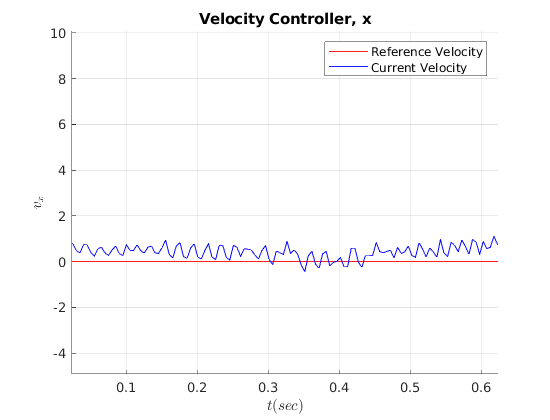
\includegraphics[width=0.95\textwidth]{figures/vel-vx-plot1.png}
	\end{minipage}
	\begin{minipage}[H]{0.45\textwidth}
		\centering
		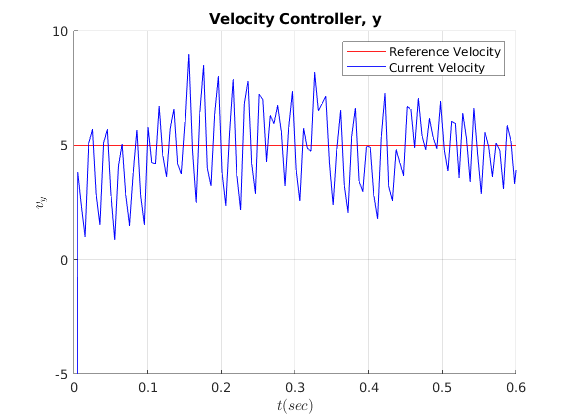
\includegraphics[width=0.95\textwidth]{figures/vel-vy-plot1.png}
	\end{minipage}
	
	\begin{figure}[H]
		\centering
		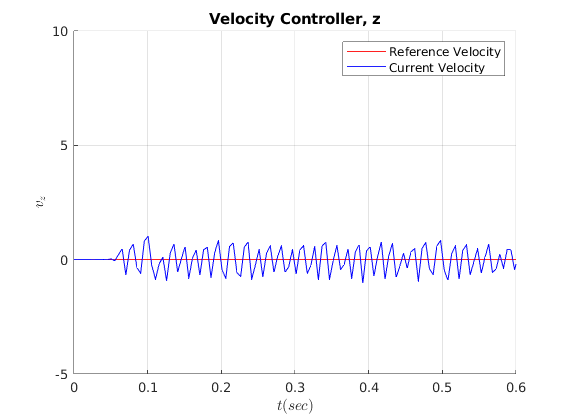
\includegraphics[width=0.45\textwidth]{figures/vel-vz-plot1.png}
	\end{figure}
	
	While there is some tuning that needs to be done on the controllers (shown by the large oscillations), it is apparent that the reference position is briefly achieved, specifically in the y axis plot, while the others remain near zero.
	\\
	
	To run:
	\begin{enumerate}
		\item \texttt{catkin\_make}
		\item \texttt{source devel/setup.bash}
		\item \texttt{roslaunch scara\_gazebo scara\_world.launch}
		\item In a new window, \texttt{rosrun scara\_pd\_controller pd\_control.py}. The controller will begin controlling all joints to their home position ($\theta_1 = \theta_2 = d_3 = 0$).
		\item In a new window, \texttt{rosservice call /scara/JointControlReference "th1\_des: X.XX th2\_des: X.XX d3\_des: X.XX"} where \texttt{X.XX} and set the robot away from any singularities.
		\item In a new window, \texttt{rosrun scara\_velocity\_controller velocity\_control.py}. The controller will begin controlling all joint velocity to achieve the predetermined EE velocity ($v_y = 5$).
	\end{enumerate}
\end{enumerate}
\end{document}



